\section{SPOT Trace vessel tracking}

Fishing grounds are determined by placing Spot Trace units on all fishing boats participating in this program. When in motion, Spot Trace units automatically report an hourly location, and when at rest for more than 24 hours, they relay daily status reports. Location and status report messages are automatically recorded in I-Fish Community, an online database running PostgreSQL with a user interface programmed in Java and analysis and reporting procedures in R and Latex.

Fishing vessels with Spot Trace units on board generate accurate data on fishing grounds and specific fishing locations within fishing grounds. Traditionally, fishing ground data were often collected from logbook data or captain interviews. However, logbook and interview data are sometimes unclear, inaccurate and can easily be falsified. The Spot Trace enables us to match catch data with exact fishing locations, while at the same time providing additional safety features on board the fishing vessels. To mitigate IUU fishing accusations, having the Spot Trace onboard can also be used as proof of legal fishing within Indonesian waters.

\section{Crew Operated Data Recording System}

Data on species and size distributions of complete catches are needed for accurate length based stock assessments. Such data on individual fishing trips are collected via Crew Operated Data Recording Systems or CODRS. This catch data is geo-referenced as the CODRS works in tandem with the Spot Trace vessel tracking system. Crews of fishing vessels are contracted to take images on project-supplied digital cameras of all fish in the catch, positioned over measuring boards. This procedure takes place when batches of fish are taken from chiller boxes on deck, before they are packed on ice in the hold. The crew photographs all the fish in this manner and at the end of the trip hands in the storage chip from the camera to a project staff who analyzes the images back at the fisheries station. Analysis of the images includes ID of the species and reading of the length of the fish as displayed on the measuring board. Double checking with owner and trader data on total catches, and comparison with weights as calculated from fish lengths, ensures that we are capturing length frequencies of the total catch. It is essential to ensure that no species or size classes are missing before analysis. If estimated catch weight from CODRS data differs more than 30% from estimates based on boat owner data, the catch is not included in the length based assessment, to remove any chance of bias.

\begin{center}
\graphicspath{{/root/R-project/IFishSnapperWPP712_713/Images/}}
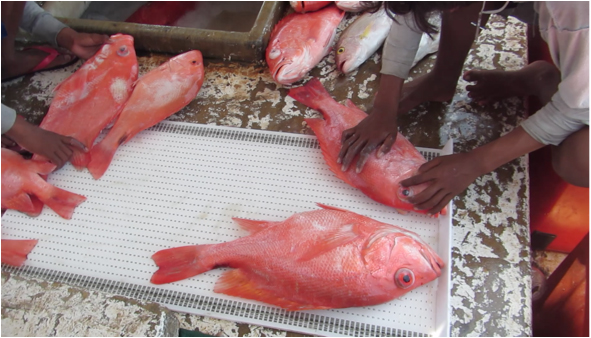
\includegraphics[scale=0.7]{codrs.jpg}

Figure 3. Fishing crew preparing fish on a measuring board.
\end{center}

\begin{center}
\graphicspath{{/root/R-project/IFishSnapperWPP712_713/Images/}}
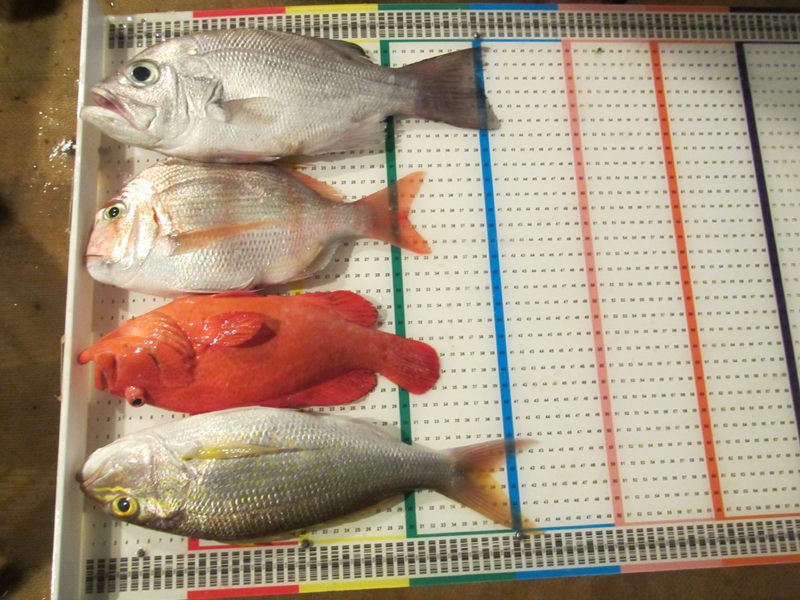
\includegraphics[scale=0.5]{codrs2.png}

Figure 4. Fish photographed by fishing crew on board as part of CODRS.
\end{center}

\clearpage
\newpage

\section{I-Fish Community}

I-Fish Community only stores data that are relevant to fisheries management, whereas data on processed volume and sales, from the Smart Weighing and Measuring System, remain on servers at processing companies. Access to the I-Fish Community database is controlled by user name and password. I-Fish Community has different layers of privacy, which is contingent on the user's role in the supply chain. For instance, boat owners may view exact location of their boats, but not of the boats of other owners.

I-Fish Community has an automatic length-frequency distribution reporting system for length-based assessment of the fishery by species. The database generates length frequency distribution graphs for each species, together with life history parameters including length at maturity (Lmat), optimum harvest size (Lopt), asymptotic length- (Linf), and maximum total length (Lmax), as well as size limits used in the trade. These "trade limit" lengths are derived from general buying behavior (minimal weight) of processing companies. The weights are converted into lengths by using species-specific length- weight relationships.

Each graph (length frequency distribution by species) is accompanied by an automated length-based assessment. Any I-Fish Community user can access these graphs and the conclusions from the assessments in real time. The report is updated daily and produces a length based assessment for the 50 most abundant target species in the fishery, based on complete catches recorded on board by fishing boat crews. The graphs show the position of the catch length frequency distributions relative to various life history parameter values and trading limits for each species.

Immature fish, small mature fish, large mature fish, and a subset of large mature fish, namely "mega-spawners", which are fish larger than 1.1 times the optimum harvest size (Froese 2004), make up the specific size groups used in our length based assessment. For all fish of each species in the catch, the percentage in each category is calculated for further use in the length based assessment. These percentages are calculated and presented as the first step in the length based assessment as follows: W\% is immature (smaller than the length at maturity), X\% is small matures (at or above size at maturity but smaller than the optimum harvest size), and Y\% is large mature fish (at or above optimum harvest size). The percentage of mega-spawners is Z\%.

The automated assessment comprises of six elements from the catch length frequencies. These elements all work with length based indicators of various kinds to draw conclusions from species specific length frequencies in the catch.

\textit{1. Proportion of immature fish in the catch.}

With 0\% immature fish in the catch as an ideal target (Froese, 2004), a target of 10\% or less is considered a reasonable indicator for sustainable (or safe) harvesting (Fujita et al., 2012; Vasilakopoulos et al., 2011). Zhang et al. (2009) consider 20\% immature fish in the catch as an indicator for a fishery at risk, in their approach to an ecosystem based fisheries assessment. Results from meta-analysis over multiple fisheries showed stock status over a range of stocks to fall below precautionary limits at 30\% or more immature fish in the catch (Vasilakopoulos et al., 2011). The fishery is considered highly at risk when more than 50\% of the fish in the catch are immature (Froese et al, 2016).

\clearpage
\newpage

IF "\% immature" is lower than or equal to 10\% THEN:\\[0cm]
"At least 90\% of the fish in the catch are mature specimens that have spawned at least once before they were caught. The fishery does not depend on immature size classes for this species and is considered safe for this indicator. This fishery will not be causing overfishing through over harvesting of juveniles for this species. Risk level is low."

ELSE, IF "\% immature" is greater than 10\% AND "\% immature" is lower than or equal to 20\% THEN:\\[0cm]
"Between 10\% and 20\% of the fish in the catch are juveniles that have not yet reproduced. There is no immediate concern in terms of overfishing through over harvesting of juveniles, but the fishery needs to be monitored closely for any further increase in this indicator and incentives need to be geared towards targeting larger fish. Risk level is medium."

ELSE, IF "\% immature" is greater than 20\% AND "\% immature" is lower than or equal to 30\% THEN:\\[0cm]
"Between 20\% and 30\% of the fish in the catch are specimens that have not yet reproduced. This is reason for concern in terms of potential overfishing through overharvesting of juveniles, if fishing pressure is high and percentages immature fish would further rise. Targeting larger fish and avoiding small fish in the catch will promote a sustainable fishery. Risk level is medium."

ELSE, IF "\% immature" is greater than 30\% AND "\% immature" is lower than or equal to 50\% THEN:\\[0cm]
"Between 30\% and 50\% of the fish in the catch are immature and have not had a chance to reproduce before capture. The fishery is in immediate danger of overfishing through overharvesting of juveniles, if fishing pressure is high.  Catching small and immature fish needs to be actively avoided and a limit on overall fishing pressure is warranted. Risk level is high."

ELSE, IF "\% immature" is greater than 50\% THEN:\\[0cm]
"The majority of the fish in the catch have not had a chance to reproduce before capture. This fishery is most likely overfished already if fishing mortality is high for all size classes in the population. An immediate shift away from targeting juvenile fish and a reduction in overall fishing pressure is essential to prevent collapse of the stock. Risk level is high."

\textit{2. Minimum size as traded compared to length and maturity.}

We use a comparison between the trade limit (minimum size accepted by the trade) and the size at maturity as an indicator for incentives from the trade for either unsustainable targeting of juveniles or for more sustainable targeting of mature fish that have spawned at least once. We consider a trade limit at 10\% below or above the length at maturity to be significantly different from the length at maturity and we consider trade limits to provide incentives for targeting of specific sizes of fish through price differentiation.

IF "TradeLimit" is lower than 0.9 * L-mat THEN:\\[0cm]
"The trade limit is significantly lower than the length at first maturity.  This means that the trade encourages capture of immature fish, which impairs sustainability. Risk level is high."

\clearpage
\newpage

ELSE, IF "TradeLimit" is greater than or equal to 0.9 * L-mat AND "TradeLimit" is lower than or equal to 1.1 * L-mat THEN:\\[0cm]
"The trade limit is about the same as the length at first maturity.  This means that the trade puts a premium on fish that have spawned at least once, which improves sustainability of the fishery. Risk level is medium."

ELSE, IF "TradeLimit" is greater than 1.1 * L-mat THEN:\\[0cm]
"The trade limit is significantly higher than length at first maturity.  This means that the trade puts a premium on fish that have spawned at least once. The trade does not cause any concern of recruitment overfishing for this species. Risk level is low."

\textit{3. Current exploitation level.}

We use the current exploitation level expressed as the percentage of fish in the catch below the optimum harvest size as an indicator for fisheries status. We consider a proportion of 65\% of the fish (i.e. the vast majority in numbers) in the catch below the optimum harvest size as an indicator for growth overfishing. We also consider a majority in the catch around or above the optimum harvest size as an indicator for minimizing the impact of fishing (Froese et al., 2016). This indicator will be achieved when less than 50\% of the fish in the catch are below the optimum harvest size.

IF "\% immature + \% small mature" is greater than or equal to 65\% THEN:\\[0cm]
"The vast majority of the fish in the catch have not yet achieved their growth potential. The harvest of small fish promotes growth overfishing and the size distribution for this species indicates that over exploitation through growth overfishing may already be happening. Risk level is high."

ELSE, IF "\% immature + \% small mature" is lower than or equal to 50\% THEN:\\[0cm]
"The majority of the catch consists of size classes around or above the optimum harvest size. This means that the impact of the fishery is minimized for this species. Potentially higher yields of this species could be achieved by catching them at somewhat smaller size, although capture of smaller specimen may take place already in other fisheries. Risk level is low."

ELSE, IF "\% immature + \% small mature" is greater than 50\% AND "\% immature + \% small mature" is lower than 65\% THEN:\\[0cm]
"The bulk of the catch includes age groups that have just matured and are about to achieve their full growth potential. This indicates that the fishery is probably at least being fully exploited. Risk level is medium."

\textit{4. Proportion of mega spawners in the catch.}

Mega spawners are fish larger than 1.1 times the optimum harvest size. We consider a proportion of 30\% or more mega spawners in the catch to be a sign of a healthy population (Froese, 2004), whereas lower proportions are increasingly leading to concerns, with proportions below 20\% indicating great risk to the fishery.

IF "\% mega spawners" is greater than 30\% THEN:\\[0cm]
"More than 30\% of the catch consists of mega spawners which indicates that this fish population is in good health unless large amounts of much smaller fish from the same population are caught by other fisheries. Risk level is low."

\clearpage
\newpage

ELSE, IF "\% mega spawners" is greater than 20\% AND "\% mega spawners" is lower than or equal to 30\% THEN:\\[0cm]
"The percentage of mega spawners is between 20 and 30\%.  There is no immediate reason for concern, though fishing pressure may be significantly reducing the percentage of mega-spawners, which may negatively affect the reproductive output of this population. Risk level is medium."

ELSE, IF "\% mega spawners" is lower than or equal to 20\%, THEN:\\[0cm]
"Less than 20\% of the catch comprises of mega spawners.  This indicates that the population may be severely affected by the fishery, and that there is a substantial risk of recruitment overfishing through over harvesting of the mega spawners, unless large numbers of mega spawners would be surviving at other habitats. There is no reason to assume that this is the case and therefore a reduction of fishing effort may be necessary in this fishery. Risk level is high.

\textit{5. Take less than nature.}

Rule number one to minimize the impact of fishing (Froese et al., 2016) teaches us to "take less than nature" by ensuring that mortality caused by fishing is less than the natural rate of mortality. We consider a fishing mortality of less than half the natural mortality to be necessary to minimize the impact of fishing. We estimated the instantaneous total mortality (Z) from the equilibrium Beverton-Holt estimator from length data using Ehrhardt and Ault (1992) bias-correction, implemented through the function bheq2 of the R Fishmethods package. We estimated the natural rate of mortality (M) using Froese and Pauly (2000) empirical formula with asymptotic length as estimated by species and an ambient water temperature at fishing depth estimated at about 20 degrees Celcius. With an asymptotic length for a snapper of about 80cm this results in an M of about 0.4, which aligns well with the mean of reported values from the literature (Martinez-Andrade, 2003). The fishing mortality F follows as the difference between total and natural mortality.

IF "fishing mortality" is greater than or equal to "natural mortality" THEN:\\[0cm]
Mortality caused by fishing is greater than or equal to the natural rate of mortality. This means that impact of fishing is severe and that fishing is unlikely to be sustainable at the current level of effort. Risk level is high.

IF "fishing mortality" is lower than "natural mortality" AND "fishing mortality" is greater than 0.5 times "natural mortality" THEN:\\[0cm]
Mortality caused by fishing is lower than the natural rate of mortality but more than half of natural mortality. This means that impact of fishing is considerable and trends in various indicators need to be watched carefully while any increase in fishing effort needs to be prevented. Risk level is medium.

IF "fishing mortality" is lower than or equal to 0.5 times "natural mortality" THEN:\\[0cm]
Mortality caused by fishing is at or below a level equal to half the natural rate of mortality. This means that impact of fishing is minimized and this fishery is currently probably operating at a sustainable level of effort. Risk level is low.

\clearpage
\newpage

\textit{6. Spawning Potential Ratio.}

As an indicator for Spawning Potential Ratio (SPR, Quinn and Deriso, 1999), we used the estimated spawning stock biomass divided by the spawning stock biomass of that population it it would have been pristine (see, for example, Meester et al 2001). We calculated SPR on a per-recruit basis from life-history parameters Z, F, K (von Bertalanffy), and Linf. We estimated Z and F as explained above and K from Lopt, using the method presented in Froese and Binohlan 2000.

In a perfect world, fishery biologists would know what the appropriate SPR should be for every harvested stock based on the biology of that stock. Generally, however, not enough is known about managed stocks to be so precise. However, studies show that some stocks (depending on the species of fish) can maintain themselves if the spawning stock biomass per recruit can be kept at 20 to 35\% (or more) of what it was in the un-fished stock. Lower values of SPR may lead to severe stock declines (Wallace and Fletcher, 2001). Froese et al. (2016) considered a total population biomass B of half the pristine population biomass Bo to be the lower limit reference point for stock size, minimizing the impact of fishing. Using SPR and B/Bo estimates from our own data set, this Froese et al. (2016) lower limit reference point correlates with an SPR of about 40\%, not far from but slightly more conservative than the Wallace and Fletcher (2001) reference point. We chose an SPR of 40\% as our reference point for high risk and after similar comparisons we consider and SPR between 25\% and 40\% to represent a medium risk situation.

IF "SPR" is lower than 25\% THEN:\\[0cm]
"SPR is less than 25\%. The fishery probably over-exploits the stock, and there is a substantial risk that the fishery will cause severe decline of the stock if fishing effort is not reduced. Risk level is high."

ELSE, IF "SPR" is greater than or equal to 25\% AND "SPR" is lower than 40\% THEN:\\[0cm]
"SPR is between 25\% and 40\%. The stock is heavily exploited, and there is some risk that the fishery will cause further decline of the stock. Risk level is medium."

ELSE, IF "SPR" is greater than or equal to 40\% THEN:\\[0cm]
"SPR is more than 40\%. The stock is probably not over exploited, and the risk that the fishery will cause further stock decline is small. Risk level is low."